% ================================= chapter 1 ================================= %
\chapter{はじめに}
\section{目的}
本実験の目的は,倒立振子系を状態空間表現を用いて安定化制御し,線形不変システムを設計することである.
具体的に,次のことを目的とする.

\begin{itemize}
    \renewcommand{\labelenumi}{(\roman{enumi})}
    \item 倒立振子が安定化制御を行っている状態において,外乱による影響で振子が傾いたとき,倒立状態に戻すことができる (不安定平衡点の安定化).
    \item 倒立振子系に一定周期のパルス入力を与え,台車を目的の変位へ移動させる.
    \item 倒立振子が入力なしで静止している状態から,台車を動かすことにより振子を振り上げ,倒立状態にする (振り上げ制御).
\end{itemize}

\section{実験装置}

\begin{figure}[htbp]
    \begin{center}
        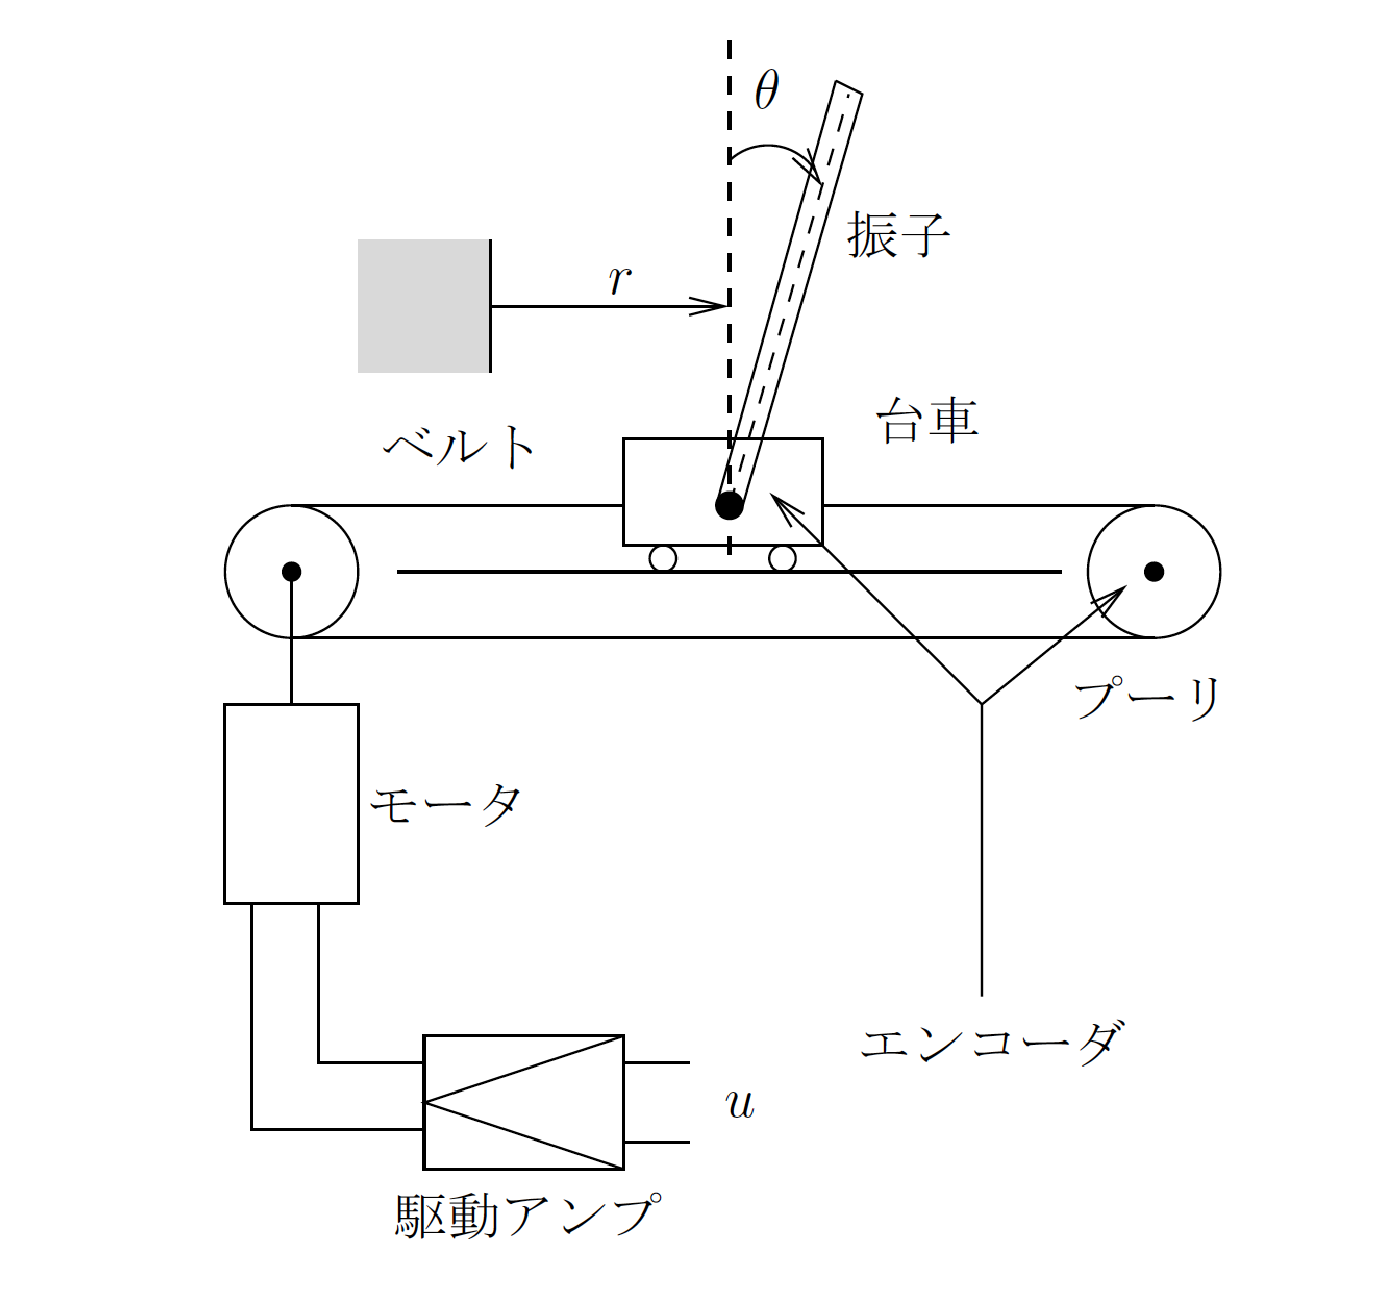
\includegraphics[width=0.6\linewidth]{model.eps}
        \caption{図\ref{pendulum}: 倒立振子系}
        \label{pendulum}
    \end{center}
\end{figure}

図\ref{pendulum}は本実験で使用する倒立振子系である.
系は,モータ,ベルト,プーリ系から成り,台車はモータからの入力によりベルト上を水平方向に動くことができる.
台車の初期状態からの変位を$r$とする.
また,鉛直方向上向きから時計回りを正の方向として,台車に取り付けられた振子が回転した角度を$\theta$とする.
ポテンショメータにより,$r$と$\theta$を測定し,入力$u$を与える.

% =============================== chapter 1 END =============================== %